\subsubsection{UC27 - Eliminazione cronologia della chat}\label{UC27}

\begin{figure}[H]
  \centering
  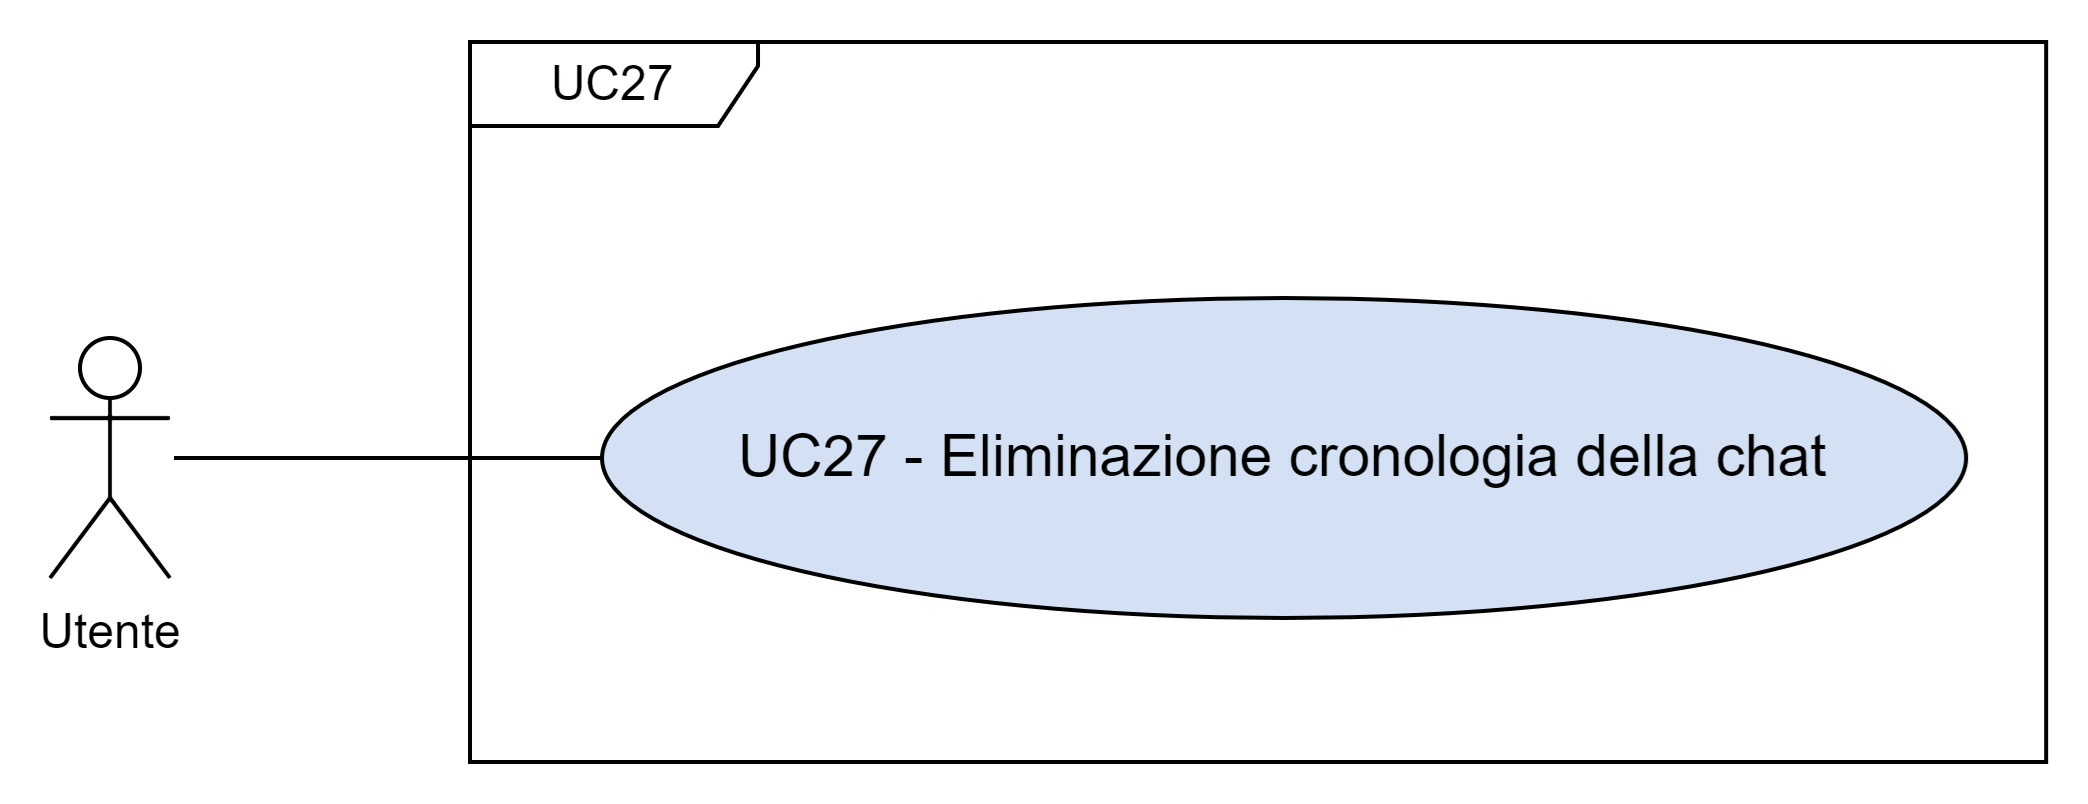
\includegraphics[width=0.90\textwidth]{assets/uc27.png}
  \caption{UC27}
\end{figure}

\paragraph*{Descrizione}
L'utente desidera eliminare la cronologia della chat, composta dalle richieste dell'utente in linguaggio naturale e dalle risposte del ChatBOT.

\paragraph*{Attori principali}
Utente

\paragraph*{Precondizioni}
\begin{itemize}
  \item L'applicazione è stata avviata con successo;
  \item È presente almeno una richiesta dell'utente e una risposta fornita dal ChatBOT.
\end{itemize}

\paragraph*{Postcondizioni}
\begin{itemize}
  \item La cronologia della chat è stata eliminata correttamente.
\end{itemize}

\paragraph*{Scenario principale}
\begin{enumerate}
  \item L'utente accede alla pagina di generazione del prompt;
  \item L'utente visualizza, all'interno della chat, almeno una richiesta in linguaggio naturale e una risposta del ChatBOT;
  \item L'utente seleziona l'opzione per eliminare la cronologia della chat;
  \item La cronologia della chat viene eliminata.
\end{enumerate}
